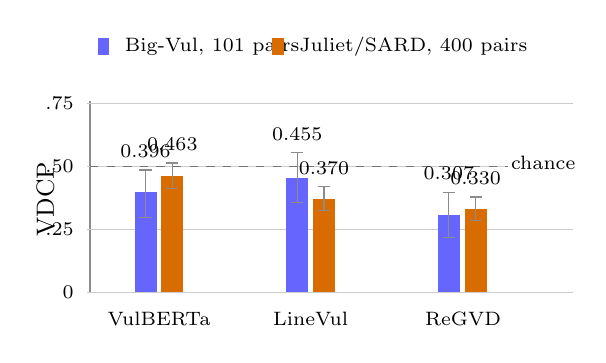
\begin{tikzpicture}[
  x=1.03cm,
  y=3.2cm,
  font=\small
]
\begin{scope}[shift={(0,-0.16)}]
\draw[black!45] (0,0) -- (5.95,0);
\draw[black!45] (0,0) -- (0,0.76);
\foreach \y/\label in {0/0,0.25/.25,0.50/.50,0.75/.75} {
  \draw[black!20] (-0.04,\y) -- (5.95,\y);
  \node[anchor=east, font=\scriptsize] at (-0.08,\y) {\label};
}
\node[anchor=center, rotate=90] at (-0.55,0.37) {VDCP};
\draw[dashed, black!55] (0,0.5) -- (5.95,0.5);
\node[anchor=west, font=\scriptsize, fill=white, inner sep=1pt] at (5.15,0.515) {chance};

% group 1: VulBERTa
\fill[blue!60] (0.55,0) rectangle (0.82,0.396);
\fill[orange!85!black] (0.88,0) rectangle (1.15,0.463);
\draw[black!45] (0.685,0.297) -- (0.685,0.485);
\draw[black!45] (0.61,0.297) -- (0.76,0.297);
\draw[black!45] (0.61,0.485) -- (0.76,0.485);
\draw[black!45] (1.015,0.413) -- (1.015,0.513);
\draw[black!45] (0.94,0.413) -- (1.09,0.413);
\draw[black!45] (0.94,0.513) -- (1.09,0.513);
\node[anchor=north, align=center, font=\scriptsize] at (0.85,-0.04) {VulBERTa};

% group 2: LineVul
\fill[blue!60] (2.42,0) rectangle (2.69,0.455);
\fill[orange!85!black] (2.75,0) rectangle (3.02,0.370);
\draw[black!45] (2.555,0.356) -- (2.555,0.554);
\draw[black!45] (2.48,0.356) -- (2.63,0.356);
\draw[black!45] (2.48,0.554) -- (2.63,0.554);
\draw[black!45] (2.885,0.323) -- (2.885,0.420);
\draw[black!45] (2.81,0.323) -- (2.96,0.323);
\draw[black!45] (2.81,0.420) -- (2.96,0.420);
\node[anchor=north, align=center, font=\scriptsize] at (2.72,-0.04) {LineVul};

% group 3: ReGVD
\fill[blue!60] (4.29,0) rectangle (4.56,0.307);
\fill[orange!85!black] (4.62,0) rectangle (4.89,0.330);
\draw[black!45] (4.425,0.218) -- (4.425,0.396);
\draw[black!45] (4.35,0.218) -- (4.50,0.218);
\draw[black!45] (4.35,0.396) -- (4.50,0.396);
\draw[black!45] (4.755,0.285) -- (4.755,0.378);
\draw[black!45] (4.68,0.285) -- (4.83,0.285);
\draw[black!45] (4.68,0.378) -- (4.83,0.378);
\node[anchor=north, align=center, font=\scriptsize] at (4.60,-0.04) {ReGVD};

\node[anchor=south, font=\scriptsize] at (0.685,0.495) {0.396};
\node[anchor=south, font=\scriptsize] at (1.015,0.525) {0.463};
\node[anchor=south, font=\scriptsize] at (2.555,0.565) {0.455};
\node[anchor=south, font=\scriptsize] at (2.885,0.430) {0.370};
\node[anchor=south, font=\scriptsize] at (4.425,0.407) {0.307};
\node[anchor=south, font=\scriptsize] at (4.755,0.388) {0.330};
\end{scope}

\fill[blue!60] (0.10,0.78) rectangle (0.24,0.85);
\node[anchor=west, font=\scriptsize] at (0.31,0.815) {Big-Vul, 101 pairs};
\fill[orange!85!black] (2.25,0.78) rectangle (2.39,0.85);
\node[anchor=west, font=\scriptsize] at (2.46,0.815) {Juliet/SARD, 400 pairs};
\end{tikzpicture}
